\documentclass[10pt, a4paper]{beamer}
\usepackage{multirow}

\usepackage[english]{babel}
\usepackage{blindtext}

\usepackage{graphicx}
\usepackage[export]{adjustbox}
\usepackage{wrapfig}

\usetheme{Berkeley}
\usecolortheme{sidebartab}

\newcommand\tab[1][1cm]{\hspace*{#1}}

\begin{document}
	\setbeamertemplate{sidebar left}{}
	\title{Progress Presentation-I}
	\subtitle{e-Yantra Summer Internship-2018 \\Machine Learning and It's Application}
	\author{Swapnil Masurekar\\Abhishek Sharma\\
	Mentors: Rutuja, Suprabha}
	\institute{IIT Bombay}
	\date{\today}
	%\addtobeamertemplate{sidebar left}{}{\includegraphics[scale = 0.3]{logowithtext.png}}
	\frame{\titlepage}

\setbeamertemplate{sidebar left}[sidebar theme]
\section{Overview of Project}
\begin{frame}{Overview of Project}
	
	\begin{itemize}
		\item Project Name : \textbf{Machine Learning and It's Application}\\
		\item Objective : To study machine learning and to work on its practical applications of Character Recognition, Automated Reply, Face Recognition along with documentation\\
		\item Deliverables : 
          \begin{enumerate}
          \item Learning ML and implement Applications
          \item Well commented code and documentation\\ 
          \end{enumerate}
	\end{itemize}
\end{frame}

\section{Overview of Task}
\begin{frame}{Overview of Task}
	\begin{tabular}{| c | l | c |}\hline
    \textbf{Task no.} & \hspace{2.9cm} \textbf{Task}  & \textbf{Deadline} \\\hline
    \multicolumn{3}{ |c| }{\textbf{Week 1}} \\
    \hline
     1 & Learning Basics of ML& 3 days \\\hline
     2 & Get familiar with Tensorflow(and python)    & 3 days \\\hline
     
     \multicolumn{3}{ |c| }{\textbf{Week 2}}  \\
     \hline
    
     3 &  Character recognition using logistic regression & 3 days \\\hline
     4 & Character recognition using neural network & 3 days \\\hline
     
     \multicolumn{3}{ |c| }{\textbf{Week 3 and Week 4}} \\
     \hline
    
     5 &  Automated Reply & 12 days \\\hline
    
     \multicolumn{3}{ |c| }{\textbf{Week 5}} \\
     \hline
         
     6 & Face Recognition & 6 days \\\hline
     
     \multicolumn{3}{ |c| }{\textbf{Week 6}} \\
     \hline
         
     7 & Documentation & 6 days   \\\hline
 
    \end{tabular}
    
\end{frame}



	

\section{Task Accomplished}

\begin{frame}{Dataset Description}
  \begin{figure}
   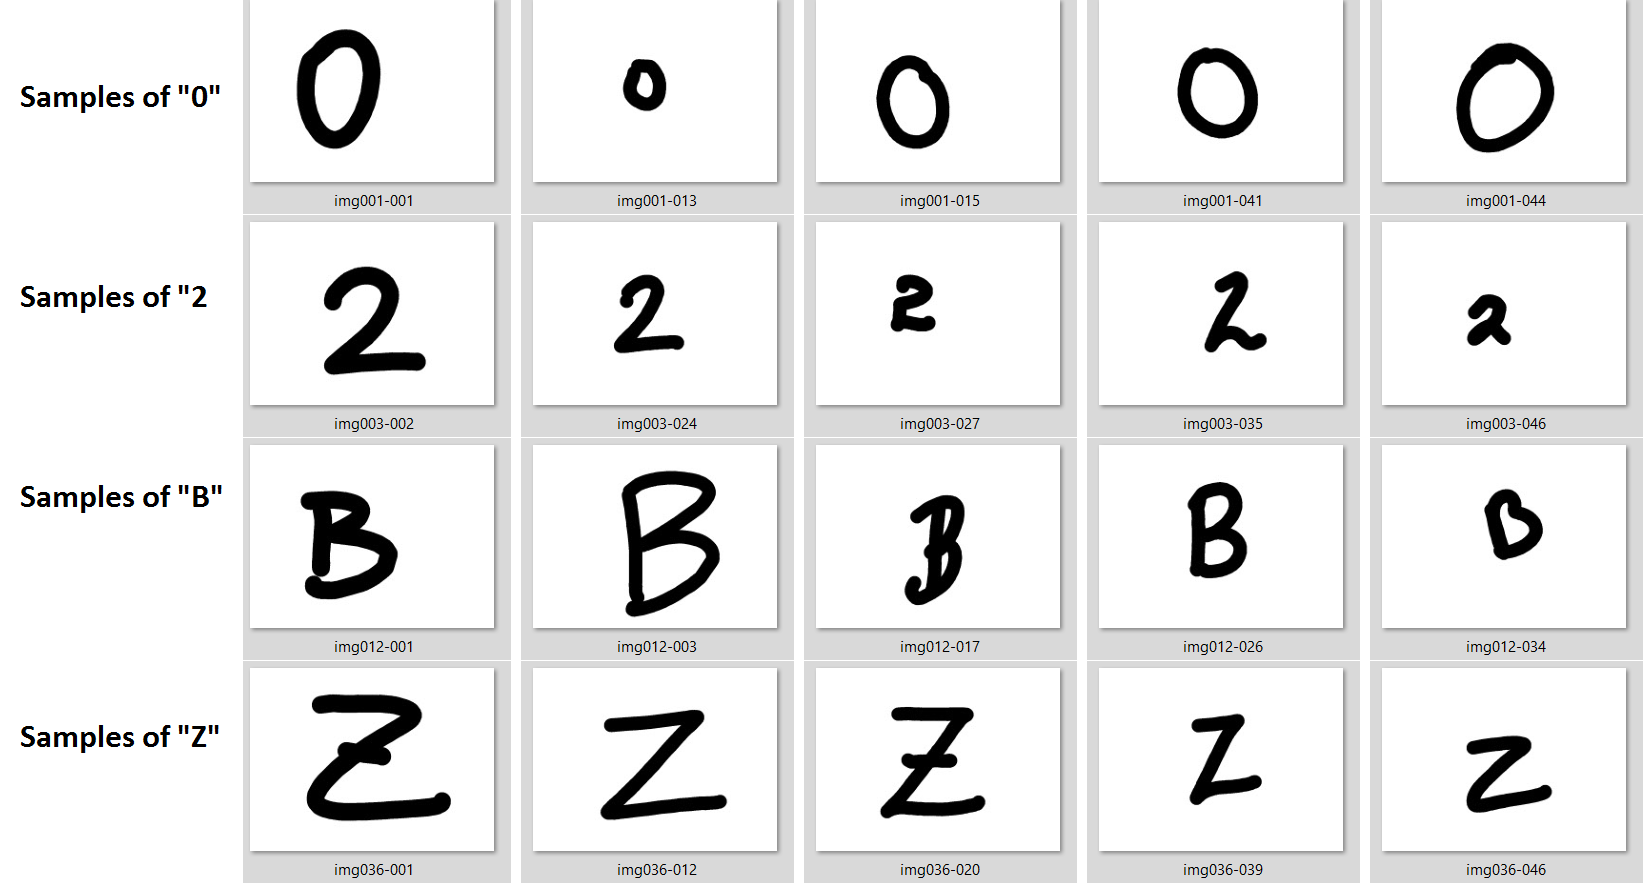
\includegraphics[height=0.72 \textheight]{dataset.png}
   \caption{Dataset of 3410 samples (55 samples of each category)}
  \end{figure}
\end{frame}

\begin{frame}{Task Accomplished}
	\begin{itemize}
		\item Image Preprocessing for recognition based on an image or a camera frame: 
	\end{itemize}
        
    \begin{figure}
 	    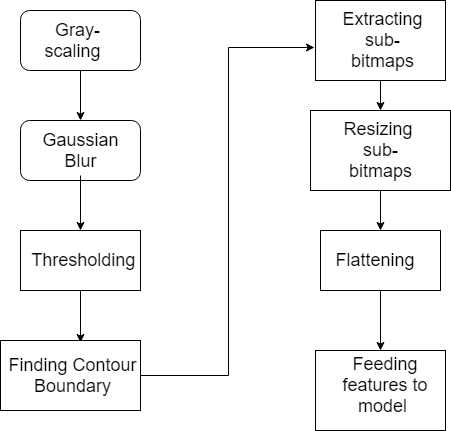
\includegraphics[height=0.65 \textheight]{Image_preprocessing_Flowchart.png}
	\end{figure}

\end{frame}



\begin{frame}{Logistic Regression}
\begin{itemize}
\item Character Recognition using Logistic Regression:\\
    \begin{enumerate}
    {\scriptsize
	\item  Formatting Dataset for detection of characters and storing the classifications and flattened images in a text file
   	\item Selecting Solver, algorithm used in the optimization problem\\

    \begin{center}
    
    \begin{table}     
    \caption{ Grid-Search Results}
      \begin{tabular}{| c | c |}
      \hline
		\textbf{Solver} & \textbf{Validation Accuracy(\%)}\\\hline
        newton-cg & 84.8516\% \\\hline
        lbfgs & 85.1402\% \\\hline
        liblinear & 83.6721\% \\\hline
        sag & 85.2901\% \\\hline
        saga & 85.5486\% \\\hline
      \end{tabular}
      \end{table}
      
    \end{center}
 
    \item k-Fold cross-validation results for model trained on English handwriting dataset (k=10):\\
    }
    
    \begin{itemize}
    {\scriptsize
    \item Mean Accuracy = 85.29\%
    \item Standard Deviation = 0.04166
    }
    \end{itemize}
	\end{enumerate}
\end{itemize} 
 \end{frame}

\begin{frame}{Artificial Neural Networks}
\begin{itemize}
\item Input-image: Flattened vector with 600 features
\item Neurons in hidden layer has uniform weights initialization and rectifier activation function associated
\item Neurons in output layer has softmax activation function
\item Now, for Real-Time data augmentation:
  \begin{enumerate}
  \item 2D array required, instead of only threshold image information in 600 feature's vector
  \item Pooling is required before flattening the images 
  \end{enumerate}
\end{itemize}
\end{frame}

\begin{frame}{Convolutional Neural Networks}
Network Structure:\\
	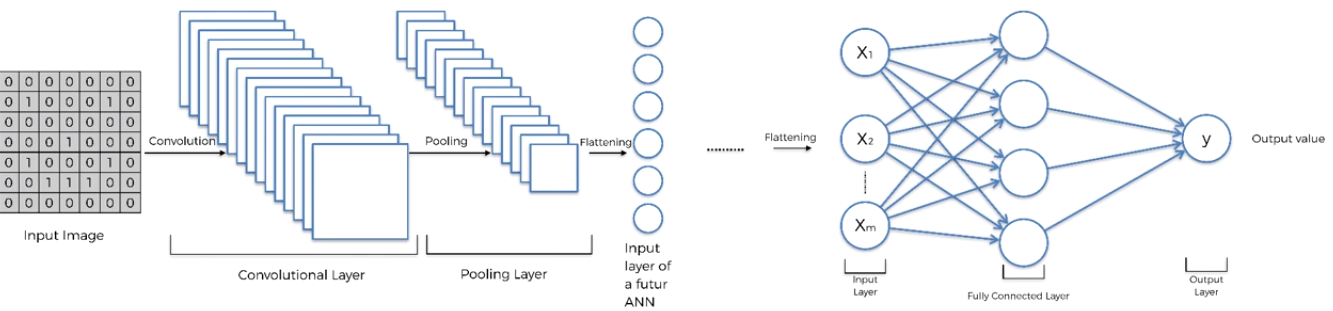
\includegraphics[height=0.34 \textheight]{conv_explanation.png}
\begin{itemize}
\item Input-image: 32x32x1 Gray-scale samples
\item 32 2x2 filters in Convolution layer
\item Rectifier Activation function
\item Softmax activation for output layer
\item Optimization score function: Categorical Cross-Entropy
\item Real-Time Data Augmentation 
\end{itemize}

\end{frame}

\begin{frame}{CNN Accuracies Plot}
% \begin{columns}

% \column{0.5 \textwidth}
% \begin{figure}
%  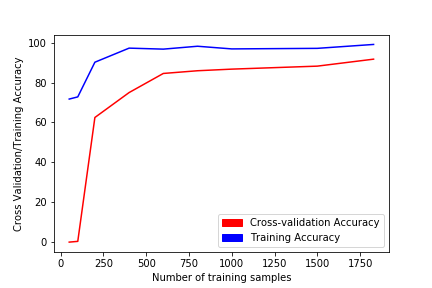
\includegraphics[height=0.48 \textheight]{NN_accuracy.png}
%  \caption{\scriptsize ANN cross-validation accuracy v/s No. of training examples}
% \end{figure}

% \column{0.5 \textwidth}

\begin{figure}
 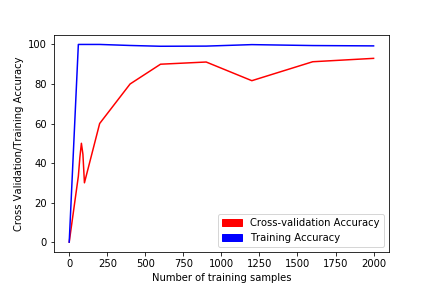
\includegraphics[height=0.6 \textheight]{sample_vs_accuracy.png}
 \caption{\scriptsize CNN cross-validation accuracy v/s No. of training examples}
\end{figure}

% \end{columns}
\end{frame}


\begin{frame}{Accuracy and Loss Variations}
\begin{columns}

\column{0.5 \textwidth}
\begin{figure}
 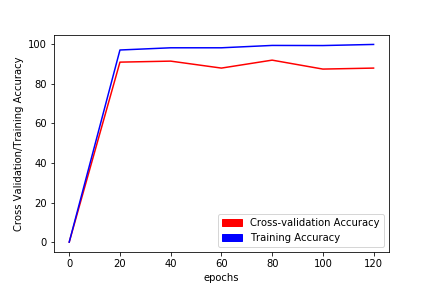
\includegraphics[height=0.48 \textheight]{epoch_vs_accuracy.png}
 \caption{\scriptsize CNN accurary variations over number of epochs }
\end{figure}

\column{0.5 \textwidth}
\begin{figure}
 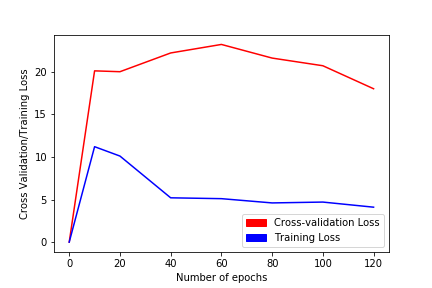
\includegraphics[height=0.48 \textheight]{epoch_vs_loss.png}
 \caption{\scriptsize CNN loss variations over number of epochs}
\end{figure}

\end{columns}
\end{frame}

\section{Results Obtained}
\begin{frame}{Convolutional Neural Network Results}
Below shown are some test Images and their predictions using CNN:
\begin{columns}

\column{0.5 \textwidth}
\begin{figure}
 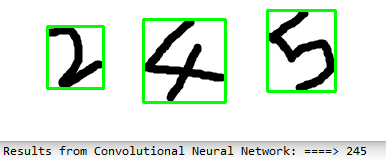
\includegraphics[height=0.26 \textheight]{test245.png}
 \caption{Rotated characters}
\end{figure}
\begin{figure}
 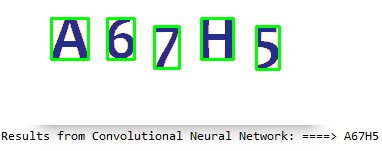
\includegraphics[height=0.26 \textheight]{testA67H5_color.png}
 \caption{Different color characters}
\end{figure}
 \column{0.5 \textwidth}
\begin{figure}
 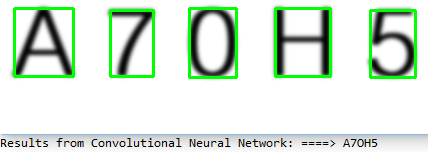
\includegraphics[height=0.25 \textheight]{testA70H5_blur.png}
 \caption{Blurred characters}
\end{figure}
\begin{figure}
 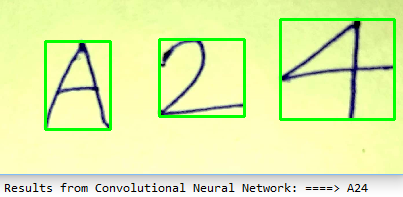
\includegraphics[height=0.27 \textheight]{testA24.png}
 \caption{Handwritten characters}
\end{figure}
\end{columns}
\end{frame}



\begin{frame}{Comparison of Logistic regression and Neural Network}
	\begin{itemize}
    	\item An ANN model without hidden layer(s) and with a sigmoidal activation function is the same as an LR model
		\item Logistic regression is a statistical approach while Neural network mimics the brains neuron network concept.
        \item Neural Networks end up solving a non-convex optimization methods while Logistic Regression end up with a Convex Optimization problem
        \item ANN will require a larger dataset for its optimization 
	\end{itemize}
\end{frame}

\section{Challenges Faced}
\begin{frame}{Challenges Faced}
	\begin{itemize}
    	\item Real-Time data augmentation in Artificial Neural Network
		\item Preprocessing the images in Handwriting Dataset and getting the feature vector 
        \item Finding the best dataset for training the model
  
	\end{itemize}
\end{frame}


\section{Future Plans}
\begin{frame}{Future Plans}
	\begin{itemize}
		\item Automated reply system for e-mails
        \item Face Recognition
	\end{itemize}
\end{frame}


\section{Thank You}
\begin{frame}{Thank You}
	\centering THANK YOU !!!
\end{frame}
\end{document}
